\documentclass[12pt]{beamer}

\usepackage[utf8]{inputenc}
\usepackage{amsmath}
\usepackage{hyperref}
\usepackage{graphicx}
\usepackage{caption}
\usepackage{subcaption}
\usepackage[style=ext-authoryear, backend=biber]{biblatex}
\addbibresource{refs.bib}

\DeclareOuterCiteDelims{parencite}{\bibopenbracket}{\bibclosebracket}

\begin{document}

\begin{frame}{Proximal Curriculum Learning \parencite{proximal}}
  \begin{itemize}
    \item Idea from educational psychology: choose tasks that are not too hard and not too easy \parencite{zpd}
    \item use \textit{probability of success} $PoS_{\theta_t}(s)$ as measure of difficulty
    \item control difficulty by adjusting start state
    \item get starting state by targeting $PoS_{\theta_t}(s) = 0.5$
  \end{itemize}
\end{frame}

\begin{frame}
  \begin{itemize}
    \item $ \mathbb{P}(s_t^0) \propto \exp(\beta \cdot PoS_{\theta_t}(s) \cdot (PoS^*(s) - PoS_{\theta_t}(s)))$
    \item $PoS^* \approx 1$: optimal policy reaches goal
    \item $PoS_{\theta_t}(s)$: approximated by rollouts or $V_{\theta_t}(s)$
    \item $\beta$: adjust sampling uniformity
  \end{itemize}
  \pause
  \begin{figure}
    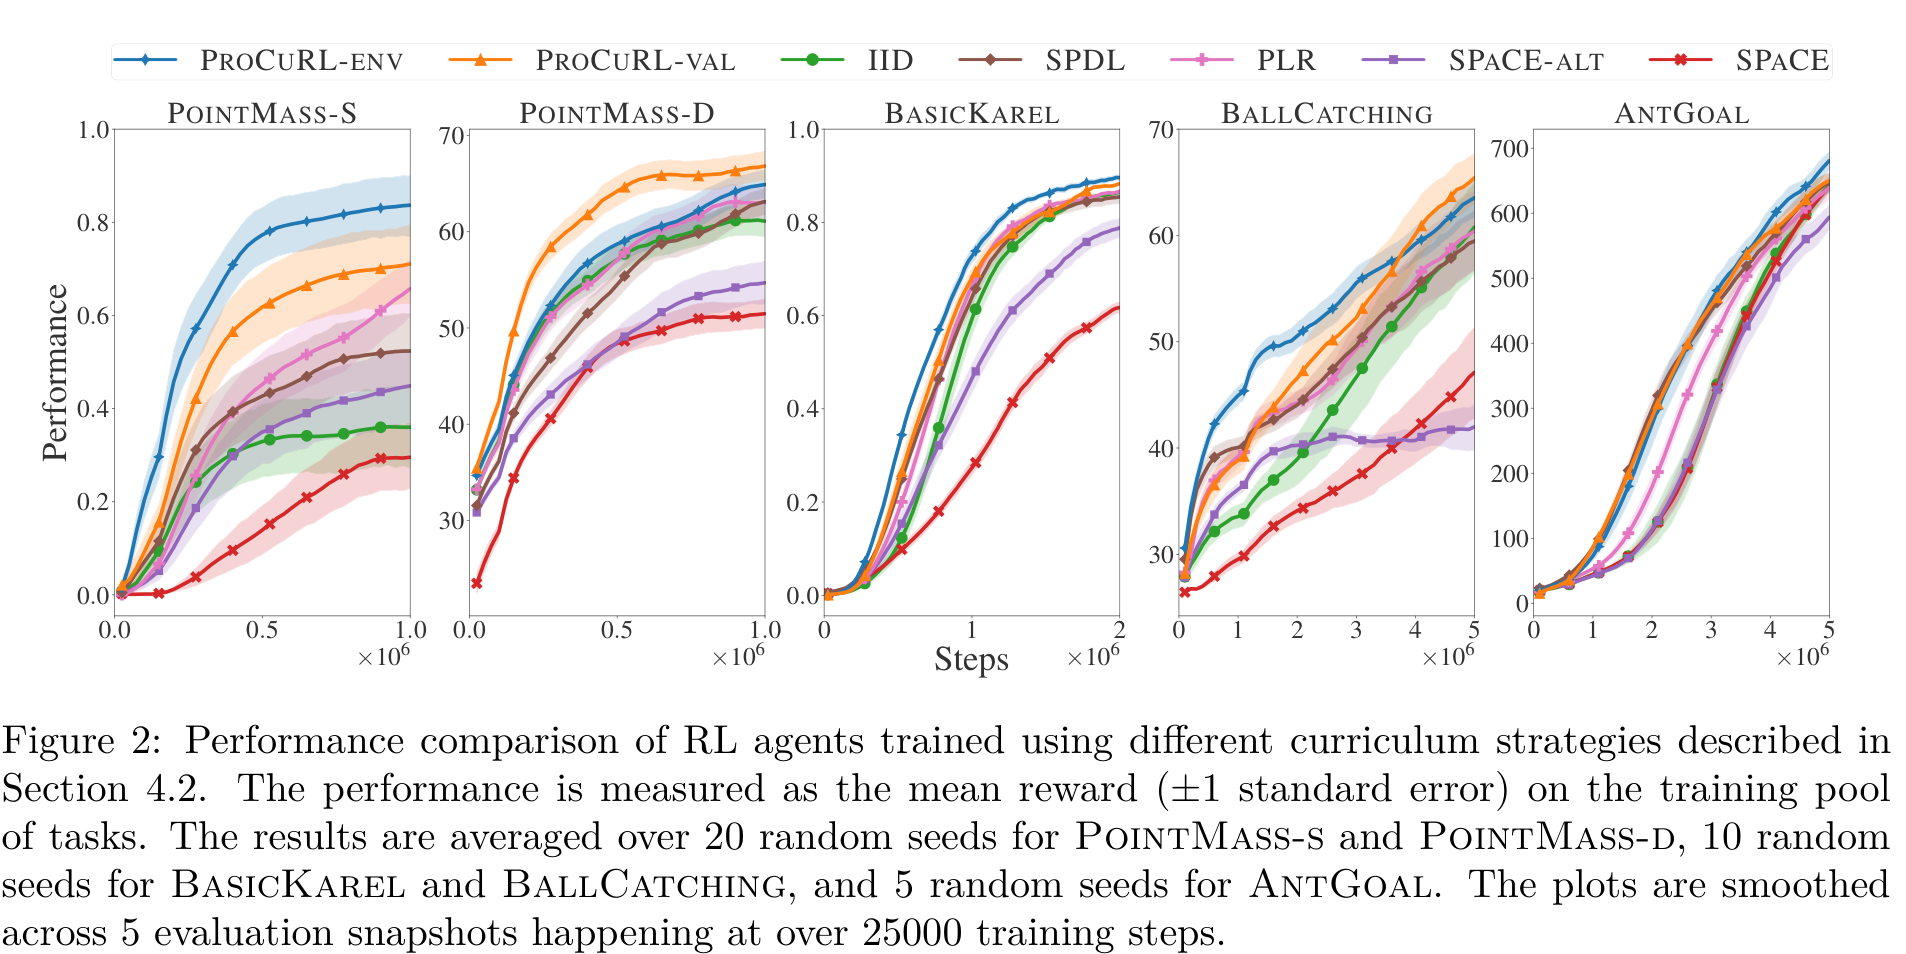
\includegraphics[width=\textwidth, height=\textheight, keepaspectratio]{./experiments.png}
    \centering
  \end{figure}
\end{frame}

\end{document}
